\newpage 

\section{Hashing \& Collisions}

In the previous section we lightly touched on the topic of hashing in Definition (\ref{def:hash_table}). 
This section will dive into more detail and difficulties collisions in hashing.

\begin{Def}[Collisions]

    A \textbf{collision} occurs when two different keys hash to the same index in a hash table.
    This is an unavoidable issue in hashing when keys begin to exceed the available indices.
\end{Def}

\begin{figure}[ht!]

    \centering
    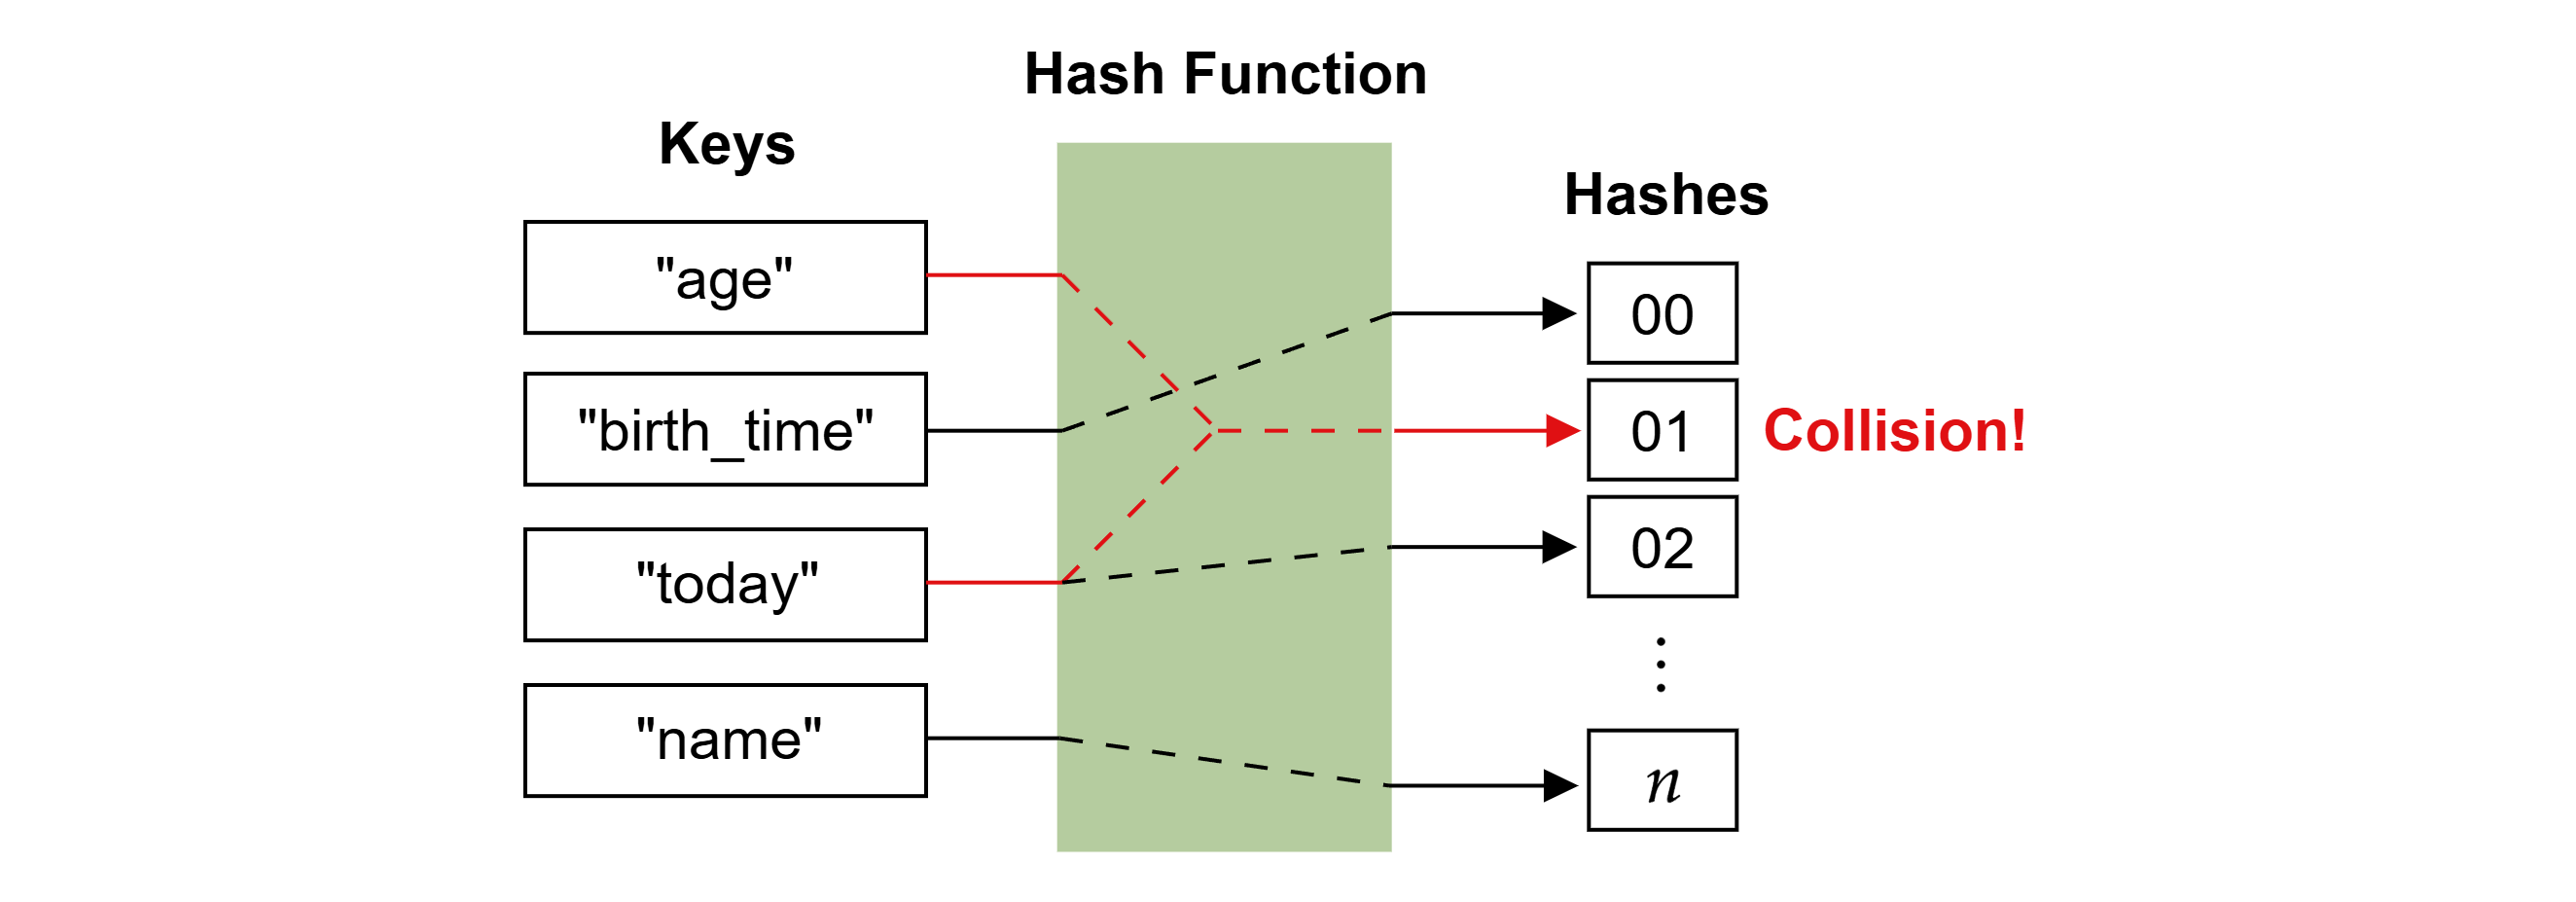
\includegraphics[width=\textwidth]{Sections/hash/collision.png}
    \caption{Four keys (`age', `birth\_time', `today', `name') go through a hash function to $n$ possible indices.
    Keys, `birth\_time' and `name', find a unique one-to-one mapping; However, `age' and `today' both hash to the same index, causing a collision.}
    \label{fig:collision}
\end{figure}
\begin{Example}[Simple Hashing Algorithm]

    Consider the hashing algorithm $H$, it takes the first ASCII value modulo the size 
    of the table. Concretely, $H(k):=\text{ASCII}(k[0])\ \%\ n$, where $n$ is the size of the table.\\

    \noindent
    Given the function $H$, we consider the following keys under a hash table of size $10$:

    \begin{itemize}
        \item \textbf{Key:} `apple' $\rightarrow$ ASCII value $=97$ $\rightarrow$ $H(\text{apple})=97\ \%\ 10 = 7$
        \item \textbf{Key:} `banana' $\rightarrow$ ASCII value $=98$ $\rightarrow$ $H(\text{banana})=98\ \%\ 10 = 8$
        \item \textbf{Key:} `bread' $\rightarrow$ ASCII value $=98$ $\rightarrow$ $H(\text{bread})=98\ \%\ 10 = 8$
    \end{itemize}
    
    \noindent
    Here, we see that `banana' and `bread' both hash to index $8$, causing a collision.
\end{Example}
One could have a superb hashing algorithm, but when space is tight, collisions are inevitable. We'll look at two particular methods for dealing with this issue.

\newpage 

\subsection{Open Addressing}
\noindent
Our first method:
\begin{Def}[Open Addressing]

    \textbf{Open addressing} is a collision resolution method where, upon a collision, the algorithm searches for the next available slot via a probing sequence.\\

    \noindent
    \textbf{Wrap Around:} the algorithm uses a modulo operation (e.g., Given a table size of 10 and request for index 12, the algorithm would use $12\ \%\ 10 = 2$).
    
    \noindent
    \rule{\textwidth}{0.4pt}

    \noindent
    \textbf{Time Complexity:} $O(n)$, where $n$ is the number of elements in the hash table. For example, say the only free index is at 0 with all other
    indices occupied. If we hash to index 1, the algorithm will have to walk all $n$ indices to find the free index at 0. Changing the probe method only switches order of indices checked, not the worst case.\\
    \textbf{Space Complexity:} $O(n)$, where $n$ is the size of the hash table (no additional space).
\end{Def}

\begin{figure}[ht!]

    \centering
    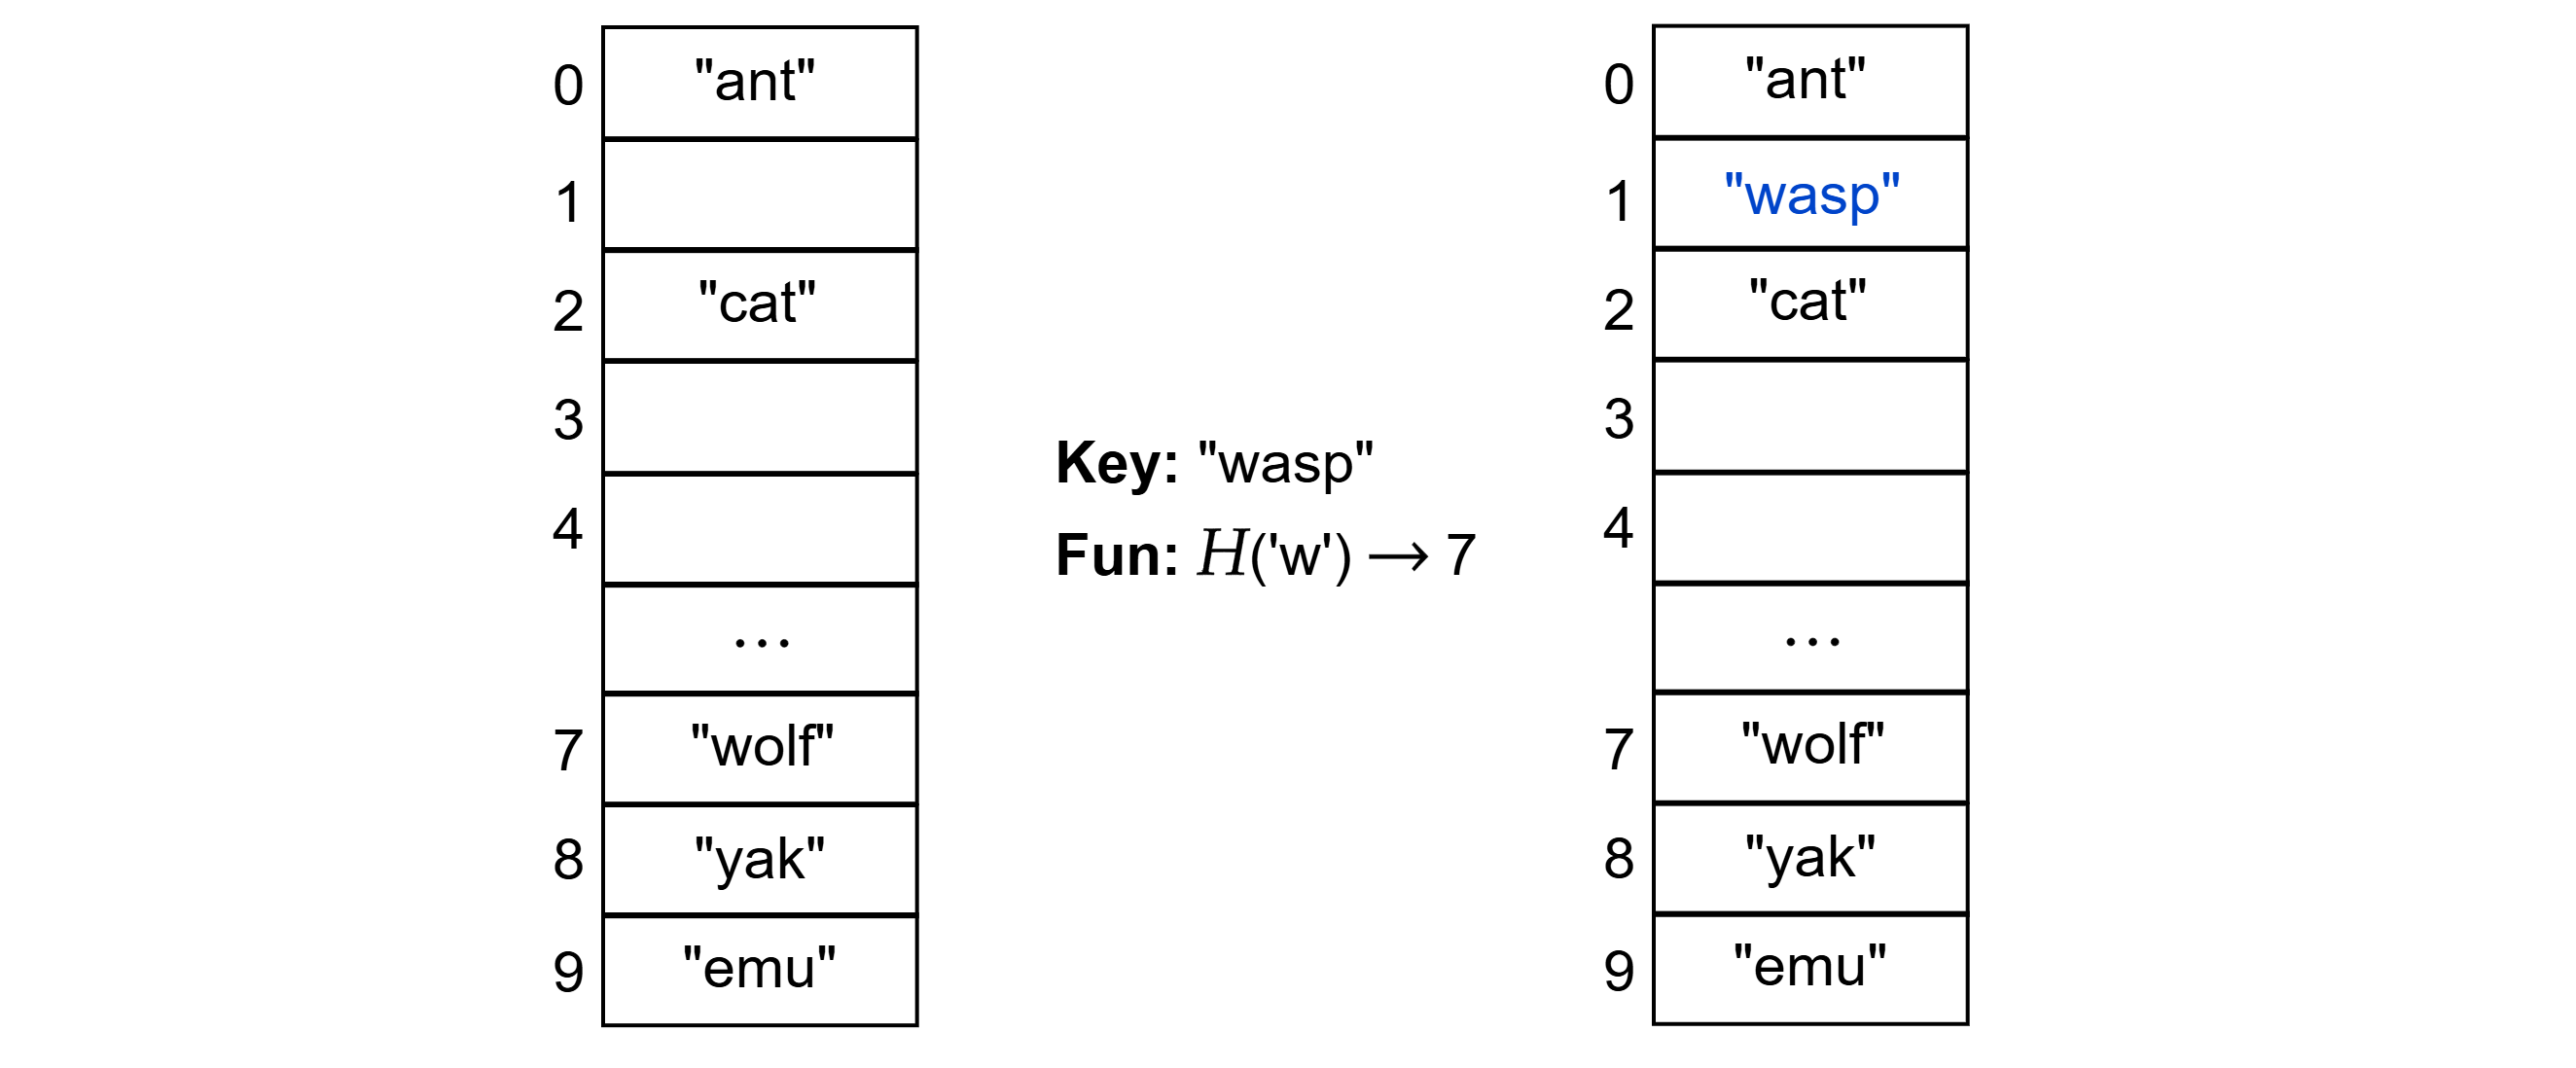
\includegraphics[width=\textwidth]{Sections/hash/open_addressing.png}
    \caption{On the left is an existing hash table of 10 elements filled with various keys. The middle shows the insertion of a new key,
    `wasp', which the function $H$ hashes to index $7$; However, index $7$ already occupied. The algorithm walks through the table, wrapping around
    to the beginning, finding a free index at 1. The right shows the final state of the hash table with `wasp' inserted at index $1$.}
    \label{fig:open_addressing}
\end{figure}

\begin{Def}[Linear Probing]

   \textbf{Linear Probing} in open addressing refers to sequentially checking each index for an available slot (e.g., Figure \ref{fig:open_addressing}).
\end{Def}

\newpage

\begin{Def}[Quadratic Probing]

    Given a universal hashing function  $H(x)$, a \textbf{quadratic probing} resolves collisions by defining,
    \[h(x,k):= (H(x) + k^2)\ \%\ n\] 
    Where $k$ defines the number of collisions, and $n$ hash table size. The algorithm may\\
    \underline{\textbf{never discover}} particular cells due to its even probing style.
    We \textbf{terminate execution} once $n$ indices have been checked, avoiding an infinite loop.
\end{Def}

\noindent
So why even use quadratic probing?
\begin{Def}[Clustering]

    \textbf{Clustering} is a phenomenon in open addressing where multiple keys form contiguous \emph{runs} of occupied indices.
    This degrades linear probing performance; Such is the main motivation behind quadratic probing.
\end{Def}

\begin{figure}[ht!]

    \centering
    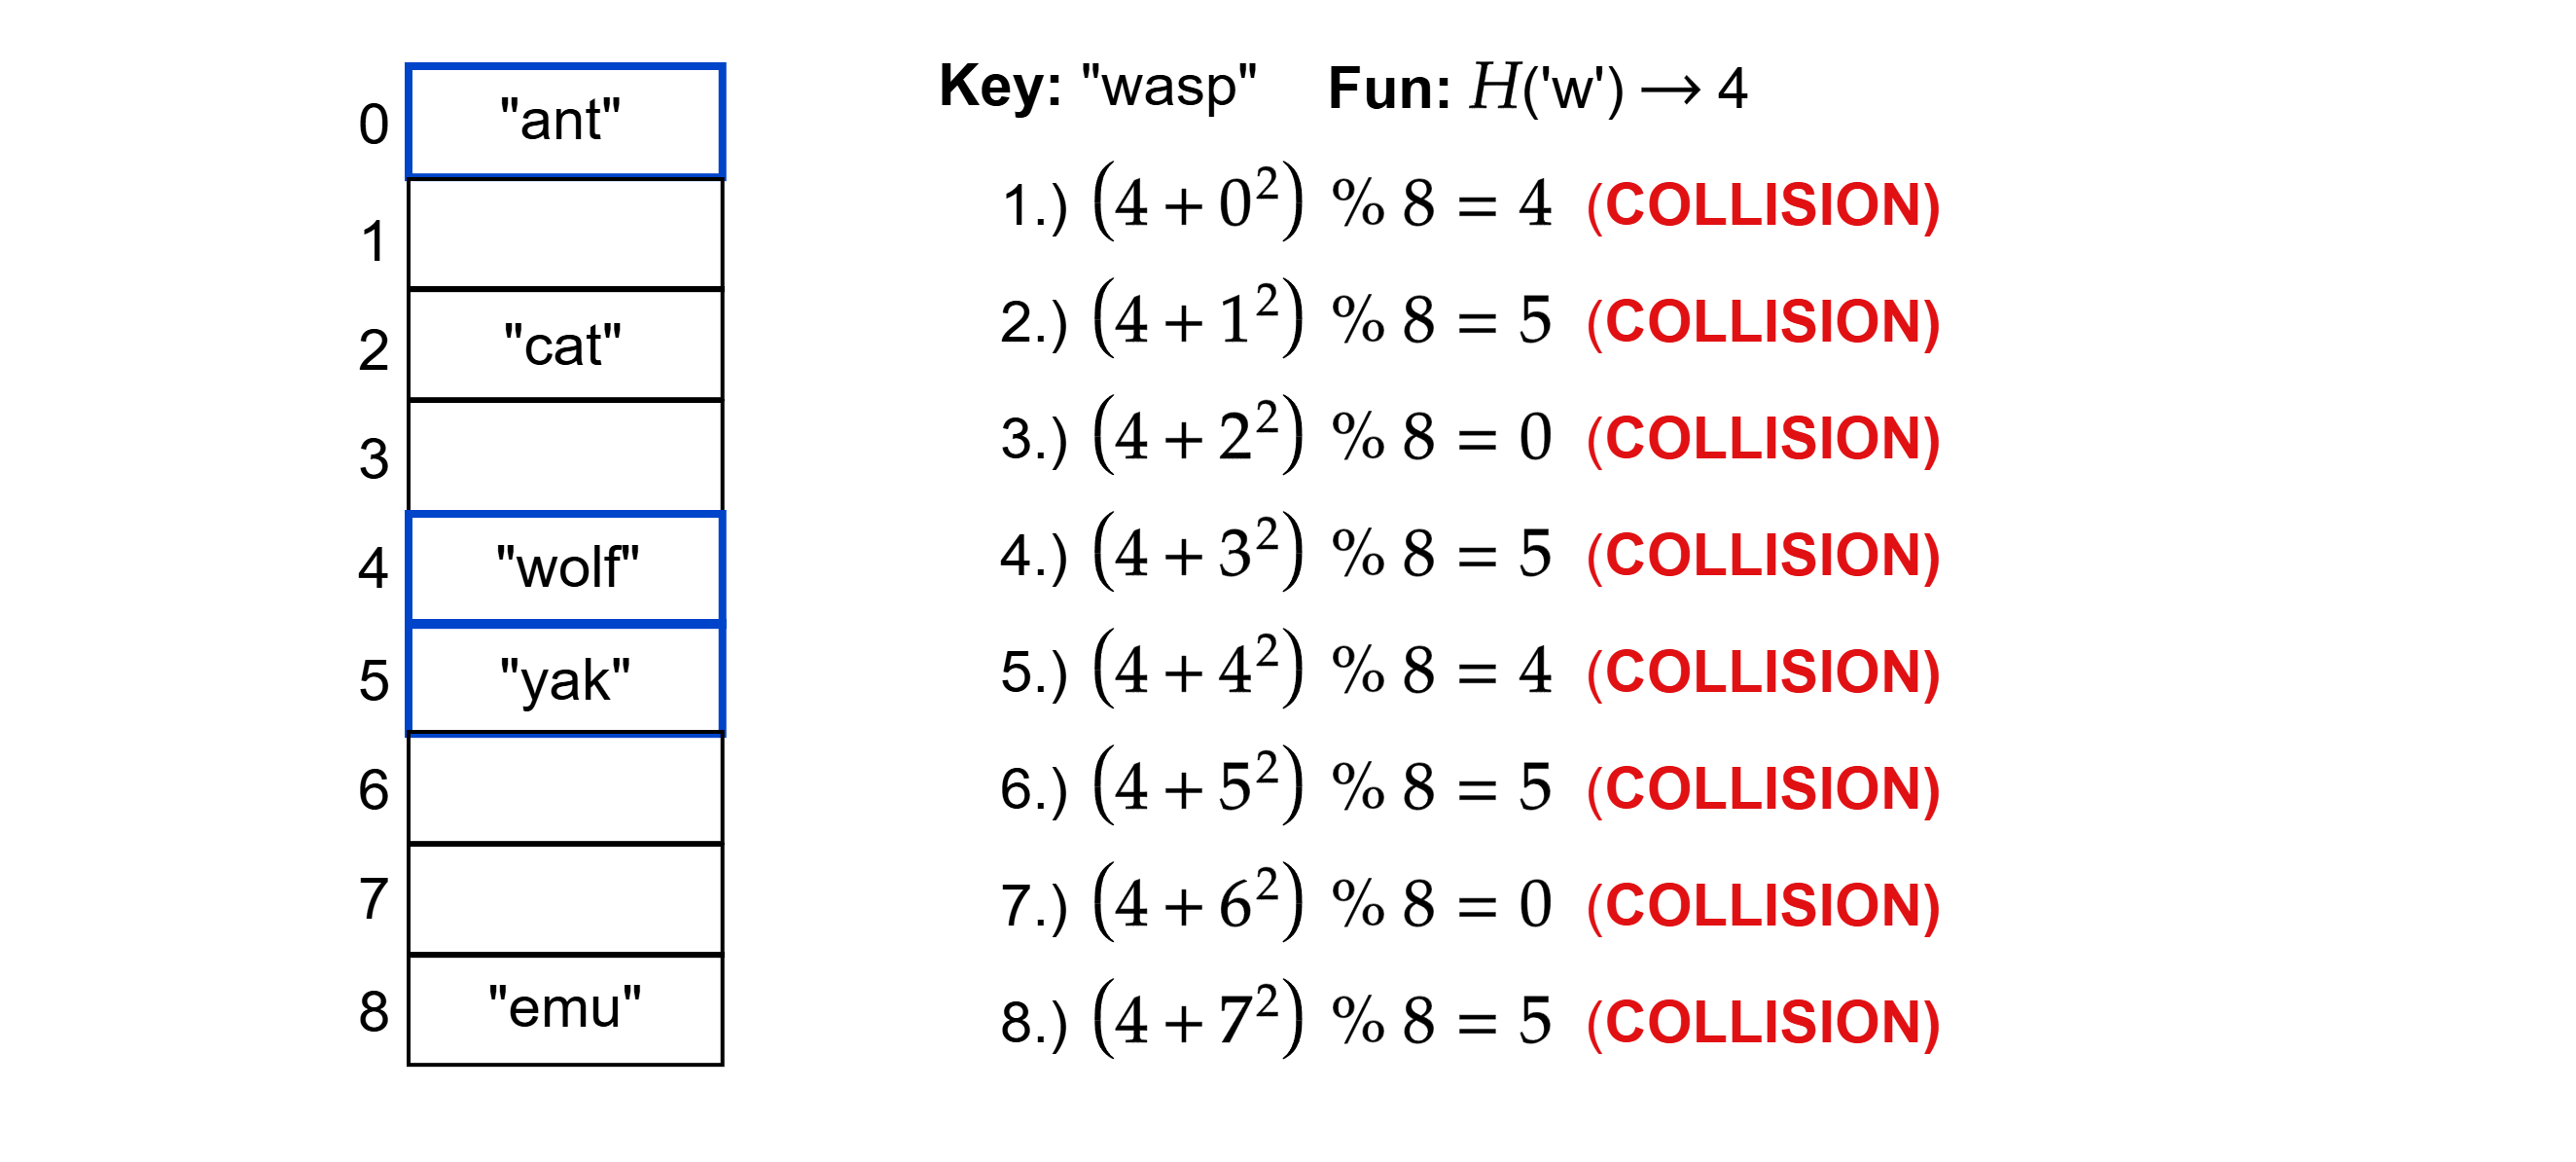
\includegraphics[width=\textwidth]{Sections/hash/quadratic_probing.png}
    \caption{On the left is an existing hash table of 8 elements. We attempt to insert a new key, `wasp', which hashes to index $4$;
    Though, 4 in occupied. The algorithm continues with $(4 + 1^2)\ \%\ 8 = 5$, which is also occupied. After some probing, it appears only indices $4, 5, 0$
    are appearing, from which are all occupied. The algorithm terminates at its $n$-th attempt with $(4+7^2)\ \%\ 8 = 5$. No spaces were found. One could imagine
    that if the table were larger or $0,4,5$ were free, the algorithm would have had better success.}
    \label{fig:quadratic_probing}
\end{figure}

\newpage 

\noindent
Another method is to have a second hash function as a backup:

\begin{Def}[Double Hashing]

  \label{def:double_hashing}
  \textbf{Double hashing} resolves collisions by using two hash functions; Given, $H_1(x)$ and $H_2(x)$ uniform hashing functions,
  we define the probe sequence $h(x,k)$ as:
  \[
    h(x,k) := \bigl(H_1(x) + k \cdot H_2(x)\bigr)\ \%\ n,
  \]
  Where $k$ is the collision count, and $n$ is the hash table size.
  $H_2(x)$ is chosen such that:
  \begin{itemize}
    \item The output hash satisfies $0 < H_2(x) < n$.
    \item It is pair-wise independent from $H_1(x)$ (i.e., not a transformation of/related to $H_1(x)$).
    \item Computationally inexpensive to evaluate.
    \item All outputs of $H_2(x)$ are relatively prime to $n$ (does not share any common factors other than $1$), ensuring all entries are probed.
  \end{itemize}
\end{Def}

\noindent 
We elaborate on the need for relatively prime numbers and why Figure (\ref{fig:quadratic_probing}) fails:
\begin{theo}[Probing Period]
 
    \label{thm:probes_period}
    A \textbf{period} defines the number of unique elements before the sequence begins to repeat. This cycle length is defined as the ratio:
    \[ \dfrac{n}{\gcd(n, H_2(x))} \]
    Where $n$ is the hash table size, and $H_2(x)$ is each output of the second hash function. We ideally want $\gcd(n, H_2(x))=1$ 
    for all $x$ to achieve a full period of $n$. Hence, if $n$ is a power of 2,
    $H_2(x)$ may uniformly provide odd numbers; Otherwise, all of $H_2(x)$ must be relatively prime to $n$ for a full period.
\end{theo}

\noindent
Without jumping too far into number theory we proceed with a proof:
\begin{Proof}[Length of Probing Period]

    \label{proof:probes_period}
    In terms of modulo, $n$ defines a cycle of $n$ elements, $0, 1, 2, \ldots, n-1$; Each element is called a \textbf{residue class}.
    E.g., 8 has residue classes $0, 1,\dots, 7$ (i.e., all possible remainders). Given a set of integers $\mathcal{H}$ (i.e., some function),
    all $\mathcal{H}_i$ need be co-prime to $n$ to exhaust all residue classes. We exclude all $\mathcal{H}_i \geq n$, as $n$'s cycle is definitively
    over (also by Definition \ref{def:double_hashing}). E.g., $1\ \%\ 8 = 1$, $9\ \%\ 8 = 1$. By contradiction, if there exists $\mathcal{H}_i$ such that $\gcd(n, \mathcal{H}_i) = d > 1$
    and $\mathcal{H}_i < n$, then $\mathcal{H}_i$ is congruent to 0 modulo $d$. Hence, $\mathcal{H}_i$ prematurely ends the cycle mapping to 0, meaning not all residue classes are visited.
\end{Proof}

